\section{Algorithms}
\label{sec:algs}

We propose a set of algorithms, collectively referred to as \mdrs, that make multicast trees robust to link failures.  
\footnote{The name \mdr is inspired by Johnny Appleseed, the famous American pioneer and conservationist known for planting apple nurseries and caring for its trees. }
\mdr runs at the OpenFlow controller with the goal of minimizing packet loss associated with link failures while ensuring that end-to-end delay requirements are satisfied.
\mdr divides into three parts: %each presented in detail in this section: 
\begin{enumerate}
	\item {\bf \pcnt algorithm: monitor and quickly detect link failures} when and where they occur inside the network (Section \ref{subsec:pcnt}).
	
	\item {\bf Precompute backup trees} that are amenable to fast installation.  In Section \ref{subsec:min-control} we formulate a new problem, \mcs, that aims to compute backup trees that
	reuse primary tree edges, prove \mc is at least NP-hard, and provide an approximation algorithm for \mc called \steiners.
	%minimize control plane signaling overhead, prove \mc is at least NP-hard, and provide an approximation algorithm for \mc called \steiners.

	\item {\bf Fast install of pre-computed backup trees} by reusing existing forwarding rules installed in the network, sharing forwarding rules among backup trees with common links, and
	in some cases pre-installing forwarding rules before link failures occur (Section \ref{subsec:install-backups}).  
	The backup trees are computed using \steiner from part (2). \pcnts, from part (1), triggers the installation of a set of backup trees.

	 %backup tree installed and shown in Figure \ref{fig:intuition-example-t2}).
	
\end{enumerate}


%to make multicast trees robust to link failures by monitoring and detecting failed links, precomputing backup multicast trees, and efficiently installing backup multicast trees after a link failure.
%As input, \mdr is given an undirected graph containing OpenFlow switches; the set of all multicast trees ($T$); the set of all active multicast flows ($F$); the length of each sampling window, 
%$w$, used to monitor links and specified in units of time; and, for each multicast flow, a packet loss condition for each link the flow traverses. For now, we restrict packet loss conditions 
%to be threshold-based that indicate the maximum number of packets that can be lost over $w$ time units. 
%The output of \mdr is a new set of precomputed backup multicast trees installed in the network and a set of uninstalled multicast trees.   All $T_i \in T$ that use the failed link are uninstalled and we call each such $T_i$ a \emph{failed multicast tree}.
%%The set of installed MTs includes each $T_i \in T$ that does not use the failed link and a backup tree for any $T_i$ that does. %does use a failed link.

%{\it TODO: write overview that unifies packet loss and E2E delay.}






%\subsection{Link Failure Detection using OpenFlow}
%\label{subsec:detection}

%missing: (a) openflow match and action, (b) flow-level measurement or packet loss at links

In this section, we propose a simple algorithm (\fls), used by \mdrs, that monitors links \emph{inside} the network to detect any packet loss.  To help explain \fls,
we use the example scenario from Section \ref{subsec:scenario} and refer to a generic multicast tree with an upstream node, $u$, and downstream node, $d$.
%Our presentation of \fl is necessarily brief but we provide additional details in Appendix \ref{subsec:pcnt}.  

\fl is run at the OpenFlow controller and provides accurate packet loss measurements that are the basis for identifying lossy links.
Informally, a lossy link is one that fails to meet the packet loss conditions specified by the controller.  We refer to such a link as \emph{failed}.
Although \mdr is ultimately concerned with meeting the per-packet \emph{delay} requirements of PMU applications, 
we use  packet loss (as opposed to delay) as an indicator for a failed link because OpenFlow provides no native support for timers.

\fl has the same input as \mdrs, specified in Section \ref{subsec:mdr}.
The output of \fl is any link that has lost packets not meeting the packet loss condition of any multicast flow traversing the link. 
In the remainder of this document, we assume all flows are multicast and just use \emph{flow} to refer to a multicast flow, unless otherwise specified.

Recall from Section \ref{subsec:openflow} that each OpenFlow switch maintains a flow table, where each entry contains a match rule 
(i.e., an expression defined over the packet header fields used to match incoming packets) and action 
(e.g., ``send packet out port $2$''). For each packet that arrives at an OpenFlow switch, it is first matched to a flow entry, $e$, based on the packet's header fields; 
then $e$'s packet counter is incremented; and, lastly, $e$'s action is executed on the packet. 
\footnote{Not all switches are necessarily OpenFlow-enabled. In fact, we anticipate that in practice many switches will not support OpenFlow. \fl still works such scenarios, as long as 
the packet counts are taken at OpenFlow switches. For ease of presentation, this section assumes all switches are OpenFlow-enabled.}
\fl uses these packet counter values to compute per-flow packet loss between switches over $w$ time units. 

%pcount(upstream_switch,downstream_switchs,nw_src, nw_dst,window_size) or pcount(upstream_switch,downstream_switchs,flow,window_size) 
\fl uses the subroutine, \pcnts, to measure the packet loss between an upstream node ($u$) and one or more downstream nodes.  For simplicity, we assume only a single downstream node, $d$. 
\pcnt does so on a per-flow basis over a specified sampling window, $w$, 
where $w$ is the length of time packets are counted at $u$ and $d$. For each window of length $w$, \pcnt computes packet loss for a flow $f$, that traverses $u$ and $d$, using the following steps:
\begin{enumerate}
	\item 
	\textbf{At $u$, tags and counts all $f$ packets}.  
	We assume, before any changes are made, $u$ uses flow entry $e$ to match and forward $f$ packets.
	\pcnt creates a new flow entry, $e'$, that is an exact copy of $e$, except that $e'$ embeds a unique identifier (i.e., the tag) in the packet's VLAN Id field.  Let this identifying number
	be $1111$.
	$e'$ is installed with a higher priority than $e$.  In OpenFlow, each flow entry has a corresponding priority specified upon its installation.
	%OpenFlow switches order flow entries based on their specified priority.  
	Incoming packets are matched against flow entries in priority order, with the first matching entry being used. 
	Thus, setting a higher priority for $e'$ than $e$, ensures that $u$ writes $1111$ in the VLAN Id field of all $f$ packets when $e'$ is installed.

	\item
	\textbf{Counts all tagged $f$ packets received at $d$.} \pcnt does so by installing a new flow entry at $d$, $e''$, that matches packets with VLAN Id equal to $1111$. 
	%in based on the VLAN tag applied at $u$.  

	\item 
	\textbf{After $w$ time units, turns tagging off at $u$.} To do so, \pcnt simply switches the priority of $e'$ and $e$ at $u$. 
	\footnote{\xxn{Unfortunately, OpenFlow does not allow a flow's priority to be modified.  As a workaround, we install a copy of $e$ called $e_c$.  We ensure that $e_c$ is given 
	a higher priority than $e'$.  Finally, we delete flows $e$. }}

	\item
	\textbf{Queries $u$ and $d$ for packet counts.} 
	Specifically, the controller uses the OpenFlow protocol to query $u$ for $e'$'s packet count value and $d$'s packet count value for $e''$.
	To ensure that all in-transit packets are considered, \pcnt waits ``long enough'' for in-transit packets to reach $d$, before reading $d$'s packet counter 
	(e.g., time proportional to the average per-packet delay between $u$ and $d$).

	\item
	\textbf{Garbage collection.}
	As a cleanup step delete $e'$ at $u$ and $e''$ at $d$.

	\item 
	\textbf{Computes packet loss.}
	The controller computes packet loss by simply subtracting $e'$'s packet count from $e''$'s. 

\end{enumerate}
In practice, \pcnt executes step (2) before step (1) to ensure that $u$ and $d$ consider the same set of packets.

%execute the actions specified by the first flow entry matching the packet's header

\pcnt introduced minimal overhead.  At $u$ and at each downstream counting switch, a copy of the flow entry corresponding to $f$ is required.  
However, these copies only persist during the duration of each \pcnt interval.


In the Figure \ref{fig:intuition-example} example, the controller uses \fl to measure the packet loss for the $a,\{e,f\}$ flow.  
We assume for link $(b,c)$ and the $a,\{e,f\}$ flow, \fl is given a maximum packet loss threshold of $10$ packets over $w$ time units.
For each sampling window of $w$ time units, \pcnt instructs $b$ to tag and count all packets corresponding to $a,\{e,f\}$. 
At the same time, $c$ is instructed by \pcnt to count the $a,\{e,f\}$ packets tagged by $b$. Then, the controller uses the OpenFlow protocol to query the packet counter values for $a,\{e,f\}$
at $b$ and $c$.  When $(b,c)$ fails, the packet counter at $c$ for $a,\{e,f\}$ no longer increments, causing a violation of $a,\{e,f\}$'s packet loss threshold for $(b,c)$.

\xxx{describe how pcount can reduce the number of necessary measurement points}

%As specified, \fl measures packet loss for each \emph{multicast flow} at each link.  These flow-level measurements may obfuscate aggregate link-level packet loss. For this
%reason, we plan to extend \fl to group flows together to enable \emph{aggregate} packet loss measurements. 
%Because OpenFlow provides native support for grouping flows and maintains packet counters for each 
%group, \fl can be easily extended to group and count packets for any subset of multicast flows traversing the same switch.


\pcnts's approach for ensuring consistent reads of packet counters bears strong resemblance to the idea of \emph{per-packet consistency} introduced by Reitblatt et al.~\cite{Reitblatt11}.
Per-packet consistency ensures that when a network of switches change from an old policy to a new one, that
each packet is guaranteed to be handled exclusively by one policy, rather than some combination of the two policies.  In our case, we use per-packet consistency to ensure that when \pcnt reads
$u$ and $d$'s packet counters, exactly the same set of packets are considered, excluding, of course, packets that are dropped at $u$ or dropped along the path from $u$ to $d$. 

\xxn{\fl is fast because it detects link failures inside the network, rather than on an end-to-end basis.  We plan to quantify how much faster \fl is than end-to-end link failure detection 
techniques.  In addition, \fl allows for link failures to be localized, whereas end-to-end techniques may not provide the necessary insight to identify and isolate the faulty link.
}

%\xxn{Advantage of in-network detection is not just the speed but also it allows us to localize the problematic links.  End-to-end detection does not provide this insight, or at least
%not as directly.}



\xxx{ $e$ matches using tuple $(src,dst,VLAN)$}

\subsubsection{\pcnt Evaluation}

\xxxx{move this section, possibly the E2E discussion to the related work section.}

{\bf Detection using end-to-end measurements.}
An alternative approach to link failure detection is to use end-to-end probes to infer packet loss rates of individual links. C\`{a}ceres et al. \cite{Caceres99} propose a maximum likelihood estimator
for loss rates of internal links based on losses observed by multicast receivers. Their model uses the inherent correlation of packet loss across multicast receivers to improve accuracy 
of their packet loss estimates.  Although impressive accuracy results are reported, the authors' simulations show that about $2000$ end-to-end probe messages are required for packet loss
estimates to converge on the true underlying packet loss rate \cite{Caceres99}.  In our problem setting, packet loss needs to be detected over small windows of time and, unfortunately,
$2000$ messages would correspond to too larger a window of time. For this reason, we deem solutions based on end-to-end measurements a poor match for our problem domain.

{\bf 7/20/13 writing from grant about plans for evaluation.}
To date, we have implemented \pcnt in the POX OpenFlow controller using the Mininet emulator and plan to further evaluate \pcnt by using our POX-based implementation to work with real
OpenFlow switches.  To provide a point of reference, we plan to implement and measure a simple SNMP-based approach for detecting link-level packet loss.  We will quantify the error rate of \pcnt 
and the SNMP-based approach as a function of the sampling window size.  We will also quantify the detection time for \pcnt and the SNMP-based approach as a function of window size. We believe our measurement study will show \pcnt  provides accurate and fast packet loss detection across all sampling window sizes, making it a superior approach for ultra- reliable data dissemination in smart grid networks


%%%%%%%%%%%%%%%%%%%%%%%%%%%%%%%%%%%%%%%%%%%%%%%%%%%%%%%%%%%%%%%%%%%%%  END OF DETECTION SECTION %%%%%%%%%%%%%%%%%%%%%%%%%%%%%%%%%%%%%%%%%%%%%%%%%%%%%%%%%%%%%%%%%%%%%%%%%%%%%%%%%%%%%%%%%%








%\subsection{Multicast Implementation} 
\label{subsec:basic}

In keeping with its role as a general framework that provides primitives for programmable networks, OpenFlow does not explicitly provide an implementation for multicast. 
Instead, we design our own multicast implementation called \bases.  \base assign a multicast IP address to each multicast group and use
this address to setup the flow tables at the multicast tree switches.  
  \footnote{Because multicast group membership is static for power grid applications (Section \ref{subsec:pmu-requirements}, 
  we simply determine the members of each multicast group by reading their static assignment from a text file.  Note that if dynamic group membership were to be required, we could 
  replace this static policy using a protocol like IGMP. }

After the controller computes a multicast tree (described in Section \ref{subsec:min-control}), $T_i = (V_i,E_i,r,S)$, \base installs a flow entry at each switch in $V_i$. The flow entry
matches packets using the group's multicast address (all other field are left as wildcards) and sends a copy of each packet out the ports corresponding to the switch's 
outgoing links in $E_i$. If a switch in $E_i$ is adjacent to a downstream host, $h_j$, in the multicast group, then the flow entry rewrites the destination layer 2 and 3 addresses of the 
packet copy sent to $h_j$ to $h_j$'s layer 2 and 3 addresses.
\footnote{Our initial plan was to use the group table abstraction described in the OpenFlow 1.1 specification \cite{OpenFlowSpec1.1} to implement multicast but, unfortunately,
as of the writing of this paper, this feature is not yet supported by the POX controller \cite{Pox} used to implement our algorithms and 
the Mininet emulator \cite{Lantz10} used in our simulations.}

% (1) mcast group assigned mcast address, (2) After mcast tree computed for mcast group, use dst address to match packets at each switch.  packets fwded out the ports corresponding to
%  tree links, rewrite address at leaf switches.  (action applied for leaf's outport)

%those of its adjacent downstream host. (these fields were previously populated with the multicast addresses).




%Another way to implement multicast in OpenFlow is to leverage existing IP multicast protocols as detailed by Kotani et al. \cite{Kotani12}.  
%In this approach, the controller assigns a unique group ID to each multicast tree and creates a group table entry, that uses the group ID, at each switch along the multicast tree.  
%Meanwhile, the sender and its first-hop switch use IGMP to set up and manage the controller-generated group IDs. Finally, the sender embeds the group ID in each multicast packet's destination 
%field, allowing for each switch in the multicast tree to identify and forward multicast packets appropriately. 



\subsection{Computing Backup Trees}
\label{subsec:min-control}

\mdr pre-computes backup trees to install after \pcnt detects a link failure.  Here we present a new problem, \mcs, and approximate solution to \mcs, called \steiners, that aim to facilitate fast
recovery by computing backup trees that maximize the number of edges common between each backup tree and its primary tree.  This reuse of primary tree edges speeds recovery from link
failures because, in SDN, this reduces the number of new flow table entries that need to be installed in the network in response to a link failure.

\mdr uses \steiner as a part of system initialization where a set of backup trees are computed for each network link, $l$; \mdr computes a single backup tree for each primary tree using $l$. 
Additionally, \steiner is used after a set of backup trees, $\hat{T}^l$, are installed in response to a link failure.  For each newly installed tree $\hat{T}^l_i \in \hat{T}^l$, \mdr computes 
a backup tree for each link in $\hat{T}^l_i$.
%recovery by minimizing control overhead (i.e., number of new flow table entries) required to install backup trees.  

%In SDNs, reusing forwarding rules which under SDN reduces the number of new flow table entries required to install backup trees.  

%\mdr uses \steiner in two scenarios. One, as a part of system 
%initialization where a set of backup trees are computed for each network link, $l$; \mdr computes a single backup tree for each primary tree using $l$.  Two, \mdr triggers the execution of 
%backup tree computations after backup trees, $T_l$, are installed in response $l$'s failure. \mdr recomputes backup trees for all primary trees as opposed to only the newly install $T_l$ trees.
%The motivation for recomputing all backup trees is that the network state -- the set of installed forwarding rules -- is 
% the entire computation (as opposed to only computing backup trees for the newly installed
%Tl trees): for each network link, l, Appleseed computes a backup MT for each MT that would be affected if l failed. Appleseed recomputes all backup MTs because installing the Tl MTs changes how flows are distributed and processed inside the network and, as a result, may adversely affect flows processed by MTs other than those in Tl. In other words, backup MTs computed before l fails may become stale when the Tl MTs are installed since the algorithms used to compute them considered an old network state in their optimization. 

\subsubsection{\mcn Problem}
\label{subsubsec:min-control}

% Existing Outline:  (a) control overhead definition + example, (b) multiple PTs need entry for each tree (c) benefits of reducing control overhead, (d) problem definition, (e) NP-hard
% Revised Outline:  (a) informal control overhead + benefits, (b) control overhead definition, (c) example, (d) problem statement, (e) NP-hardness outline
%control overhead definition + example, (b) multiple PTs need entry for each tree (c) benefits of reducing control overhead, (d) problem definition, (e) NP-hard 
% make sure handle 1 message per flow assumptio

\mc considers backup trees that maximize reuse of primary tree edges.  Recycling primary tree edges allows the SDN controller, when generating the forwarding rules for multicasting 
packets using the backup tree, to use primary tree rules already installed in the network rather than install new ones.
%Recycling primary tree rules reduces the number rule installation messages, referred to as control messages, the controller must send network switches. 
This speeds recovery in cases where backup trees are installed \emph{after} a link failure is detected and reduces the number of flow table entries pre-installed at switches (control state) 
when backup trees are installed \emph{before} a link failure occurs.  
Reducing control state is especially important with OpenFlow because OpenFlow switches can only store a limited number of flow table entries (see Section \ref{subsec:openflow}).
\footnote{Following from our assumption that a single link fails at-a-time, \mc assumes that all other links besides the failed one, $l$, satisfy packet loss requirements. }
%\footnote{Our \mc description implies that all other links besides the failed one, $l$, satisfy packet loss requirements. This follows from our assumption that only a single link fails at-a-time.}

For the primary tree $T^l_i = (V^l_i,E^l_i,r,S)$ and its backup $\hat{T}^l_i=(\hat{V}^l_i,\hat{E}^l_i,r,S)$, we define a binary variable $c_v^l$ for all $v \in \hat{V}_i^l$. 
If $v$ has exactly the same predecessors (outgoing edges) in $T^l_i$ and $\hat{T}^l_i$, then $c_v^l$ takes value $0$.  Otherwise, $c_v^l=1$.  
%Using  $c_v^l$, define: %Define multicast recycling, for the $T^l_i$,$\hat{T}^l_i$ pair as:
For the $T^l_i$,$\hat{T}^l_i$ pair define:
\begin{eqnarray}
\label{eqn:control-overhead}
 C_i^l &=&  \sum_{\forall v \in \hat{V}_i^l} c_v^l 
\end{eqnarray}
For our purposes, $C_i^l$ is the number of new rules (i.e., non-recycled primary tree rules) needed to install $\hat{T}^l_i$.

Consider the example in Figure \ref{fig:intuition-example} where $(g,l)$ fails. The green backup tree, $\hat{T}_b$, shown in Figure \ref{fig:intuition-example-t2}, has $C_b =2$ because 
a new forwarding rule is required at $b$, and $f$ to account for the new outgoing links at each node. $\hat{T}_c$, in blue, has
only one link, $(m,l)$ not in $\hat{T}_c$'s primary tree. As a result, $C_c =3$.

Our \mc problem definition below references a modified version of the Steiner tree problem, called the \arbor problem \cite{Charikar98}. As input \arbors, is given 
a directed graph $G=(V,A)$, a root vertex $r$, and a set of terminals, $S$. An arborescence is defined as a tree directed away from $r$ that spans $S$.  \arbor aims to find a minimum cost 
arborescence, called a Steiner arborescence or directed Steiner tree. We denote $SA_i(G) = (V,E,r,S)$ as the $ith$ Steiner arborescence computed over directed graph, $G$, .

We use the following formulation for the \mc problem: 
\begin{itemize}

	%\item  \underline{Input}: $(G,T,l)$ where $G=(V,E)$ is directed graph, $T=\{T_1,T_2, \dots T_m\}$ where each $T_i \in T$ is a primary tree, and $l \in E$.
	\item  \underline{Input}: $(G,T^l,l,\alpha)$ where $G=(V,E)$ is a directed graph, $T^l=\{T_1^l,T_2^l, \dots T_k^l\}$ where each $T_i^l \in T^l$ is a primary tree that uses $l$, 
	$l \in E$, and $\alpha \geq 1$. 
	%computed using the directed Steiner tree approximation algorithm described by Charikar et al. \cite{Charikar98}, and $l \in E$.


	\item \underline{Output}: A backup tree for each primary tree using $l$. This set of backup trees, $\hat{T}^l = \{\hat{T}^l_1,\hat{T}^l_2,\dots,\hat{T}^l_k\}$:
		\begin{equation}
		\label{eqn:mc-obj-function}
		\begin{aligned}
			& {\text{minimize}}
			& & \sum_{1 \leq i \leq k} C^l_i \\
			& \text{subject to}
			& & w(\hat{T}^l_i) \leq \alpha \cdot w(SA_i(G')), \;  \forall \hat{T}^l_i \in \hat{T}^l \\
		\end{aligned}
		\end{equation}
		where $G'=(V',E')$ such that $E' = E - \{l\}$ and $w(\hat{T}^l_i)$ is the sum of $\hat{T}^l_i$'s link weights.	
		\footnote{We assume $\hat{T}^l_i$, satisfies all per-packet delay and loss requirements if $l \notin \hat{T}^l_i$ and $w(\hat{T}^l_i) \leq \alpha \cdot w(SA_i(G'))$}

\end{itemize}   % (a) assumes all other links up, (b) C^l defined between pt and bt, point shall revisit later in approx, (c) \alpha keeps tree from growing too larger
The objective function maximizes the reuse of primary tree edges, while $\alpha$ bounds how large the backup tree can grow as consequence of minimizing $C^l_i$.  When applied to our
problem scenario this formulation reduces the number of installation rules by reusing rules already installed in the network, under the constraint that the 
backup tree does not become too large to meet the end-to-end latency requirements. 
By defining $G'$ as a copy of $G$ with the failed link removed from $G$, we are assuming that all links in $G$ besides $l$ are operational.  For
our purposes, this amounts to assuming that all non-$l$ links have packet loss rates less than their threshold. %below the satisfy their packet loss rate condition.  

Notice that we have defined $C^l_i$ in Equation \ref{eqn:control-overhead} on a per-backup tree basis where for backup tree $\hat{T}^l_i$, $C^l_i$ is a relationship defined strictly between 
$\hat{T}^l_i$ and its primary tree $T^l_i$ (there are no constraints specified across any other primary or backup tree). 
%\footnote{This simplification is reasonable for our OpenFlow-based application of \mcs. In cases where multiple backup trees require a new forwarding rule at the same switch, $v$, a separate
%forwarding rule must be installed (even if these backup trees have exactly the same predecessors at $v$) for each of these backup trees because under our multicast implementation, 
%\bases, each forwarding rule matches packets using the tree's multicast address. }
As a result, the globally optimal solution for \mc  (i.e., the optimal set of backup trees for a single link)  can be found by computing the optimal backup for each primary tree in isolation
and then taking the union of these solution We shall revisit this important property when describing our approximation algorithm for \mcs.

\begin{theorem}
\label{thm:mc-npc}
\mc is at least NP-hard.
\end{theorem}
\begin{proof}
The details of our proof can be found in Appendix \ref{sec:mc-npc}. This proof shows that \mc is NP-hard even when considering just a single backup tree.  The proof demonstrates that
in some cases an optimal solution to \mc requires a solution to \arbors, a problem known to be NP-hard.  This proves \mc is NP-hard when considering a single backup tree and therefore
the general \mc problem for $k$ backup trees must at least be NP-hard. 
\end{proof}


%to derive a globally optimal solution for \mcs.  
%Notice that we have defined the control overhead as the difference between the directed edges from the backup tree and its corresponding primary tree.  This formulation
%is convenient because for a given link, $l$, we can solve \mco seperately for each directed tree using $l$ and then simply take the union of these solutions to derive a 
%globally optimal solution for \mc (for $l$).  




\subsubsection{\steinern Approximation Algorithm}
\label{subsubsec:steiner-approx}

\steiner is a simple approximation algorithm for \mc that manipulates link weights to encourage each backup tree to reuse primary tree edges.
For each link $l$,  \steiner separately computes a backup tree for primary tree using $l$ and then returns the union of these computed trees. 

%Our \mc approximation algorithm, \steiners, computes each backup tree for link $l$ separately and then returns the union of these computed trees. 
%\steiner manipulates link weights to encourage each backup tree to reuse primary tree edges. 

%\steiner leverages the \arbor approximation algorithm from Charikar et al. \cite{Charikar98}.  Their approximation algorithm computes a bunch: a subgraph 
%formed by taking the shortest path from the root to an intermediate vertex, $j$, and the union of shortest paths from $j$ to the terminal nodes.  
\steiner leverages the $\sqrt{s}$ \arbor approximation, where $s$ is the number of terminal nodes, from Charikar et al. \cite{Charikar98}. Their approximation algorithm computes bunches, 
where a \emph{bunch} is a subgraph formed by taking the shortest path from the root to an intermediate vertex, $i$, and the union of shortest paths from $i$ to the terminal nodes.  
The algorithm produces the bunch with best \emph{density} -- density is the average cost of connecting a terminal node with the root -- as its approximation.   The lowest density bunch can 
easily be computed in polynomial time: a brute-force approach that tries all possible nodes as the intermediate vertex yields an $O(ns^2 \log s)$ time algorithm. 
%where $s$ is the number of terminal nodes.  The authors prove this is a $\sqrt{s}$ approximation.


%\steiner leverages the \arbor approximation algorithm from Charikar et al. \cite{Charikar98}.  Their approximation algorithm recursively finds ``bunches'', where a bunch is a subgraph 
%formed by taking the shortest path from the root to an intermediate vertex, $j$, and the union of shortest paths from $j$ to a subset of the terminal nodes.  
%Th%e overall solution is the union of each bunch.  %We denote $B_i(G) = (V,E,r,S)$ as the $ith$ Steiner arborescence computed over directed graph, $G$, using this algorithm.
%\footnote{In our work, the initial set of primary trees (i.e., the primary trees used before any link failures) are computed using the Steiner arborescence approximation from \cite{Charikar98}.}

%Our approximation algorithm for \mc solves computes for each $T_i^l \in T^l$ and then returns the union of these results. 
%We leverage the Steiner arborescence approximation described in \cite{Charikar98} to approximate \mcos.  Abusing notation, we refer to the \mco primary tree as $T^l$ and its backup as $\hat{T}^l$.  

Given $(G,T^l,l,\alpha)$, for each $T_i^l \in T^l$ \steiner uses the following two-step procedure to compute $\hat{T}^l_i$:
\begin{enumerate}
	
	\item Make a copy of $G$ called $G'=(V',E')$ and remove $l$ from $E'$.  Set the link weight of each $e \in T^l_i$ to $0$ and the link weight of $e \notin T^l_i$ to $1$. 

	\item Run the \arbor approximation, using the brute-force approach described above, over $G'$ and set $\hat{T}^l_i$ to be the result.
	If $\hat{T}^l_i$ satisfies the Equation \ref{eqn:mc-obj-function} constraint, return $\hat{T}^l_i$ as the solution.  Otherwise, return False. 
	%Otherwise, compute the backup tree from scratch -- run the \arbor approximation 
	%over a copy of $G$ that uses $G$'s original link weights and has link $l$ removed -- and return this result.

\end{enumerate}
Setting the primary tree link weights to $0$ in Step (1) allows the \arbor approximation algorithm to use any primary tree edge without penalty (i.e., adding cost to the 
backup tree) and so encourages reusing primary tree edges.  If \steiner returns False in Step (2) either $\alpha$ must be made larger or a new multicast tree should be computed from
scratch that satisfies the tree size constraint.

In Figure \ref{fig:intuition-example}, \steiner uses $f$ as the the intermediate node for $\hat{T}_b$, yielding density of $2$ (the cost of connecting terminals $p$,$q$,$r$, and $s$ to the 
root is $2$).   The bunch for $\hat{T}_c$ is formed using $m$ as the intermediate node with density $0.4$: the cost of connecting $r$ and $s$ to the root is $1$ and $t$,$u$, and $v$ connect
with the root at $0$ cost. 






\subsection{Installing Backup Trees}
\label{subsec:install-backups}

We are now ready to describe the last part of \mdrs, installing backup trees.  %(like the ones computed by \steiners): \pre and \posts.  
Installing a backup tree is a two-step process. First, the flow entries that forward packets along the backup tree are generated.  Second, the 
controller signals the necessary switches to install the generated forwarding rules.  Here we introduce two such installation algorithms, \pre and \posts.
Both algorithms compute forwarding rules for a single backup tree at-a-time and so
our description of each algorithm (with some abuse of notation) refers to a generic primary tree, $T^l = (V^l,E^l,r,S)$, and its backup tree for $l \in E^l$, $\hat{T}^l=(\hat{V}^l,\hat{E}^l,r,S)$.  

{\bf \post \textsc{Algorithm.}}
First, \post determines which nodes require a new forwarding rule. % to install the backup tree.
 In cases where $\hat{T}^l$ and $T^l$ use exactly the same outgoing links of a common node, $u$, we say
$\hat{T}^l$ can ``reuse'' $T^l$'s forwarding rule at $u$;  since $T^l$'s forwarding rule is already installed at $u$, no new forwarding rule (for $\hat{T}^l$) needs to be installed. % at $u$.
Forwarding rules are only required at any $v \in \hat{V}^l \setminus V^l$ and at each $v \in V^l \cap \hat{V}^l$ with different outgoing links in $\hat{T}^l$ and $T^l$.  We refer to this
set of nodes as $B^l$. 

Consider $T_b$ and $\hat{T}_b$ in the Figure \ref{fig:intuition-example} example. Because $T_b$ and $\hat{T}_b$  share the same outgoing links at $l$ and $k$
$\hat{T}_b$ can reuse $T_b$'s flow entry at each of these nodes, whereas new forwarding rules are required at $b$ and $f$.

%Later in the document, we refer to the flow entries generated by \base as \emph{basic} flow entries
Second, \post pre-computes a \emph{basic} flow entry for each $b \in B^l$.  Like the flow entries \base computes (see Section \ref{subsec:basic}), a basic flow
entry, for a multicast tree $T_i$ and $u \in V_i$, matches packets using $T_i$'s multicast address and has instructions to send matching packets out the correct ports at $u$. 
%The ports are correct if the outgoing links corresponding to $e_u$'s outports are in $T^l$.
Lastly, when $l$ fails, the \post signals each $b \in B^l$ to install the pre-computed basic flow rule.
%The nodes are signalled sequentially, in bottom-up order, starting
%with the most downstream node in $U$. Bottom-up signaling ensures that each $u \in U^l$ has a matching flow entry when $\hat{T}^l$ packets arrive.


%\begin{figure}
%  \centering
%   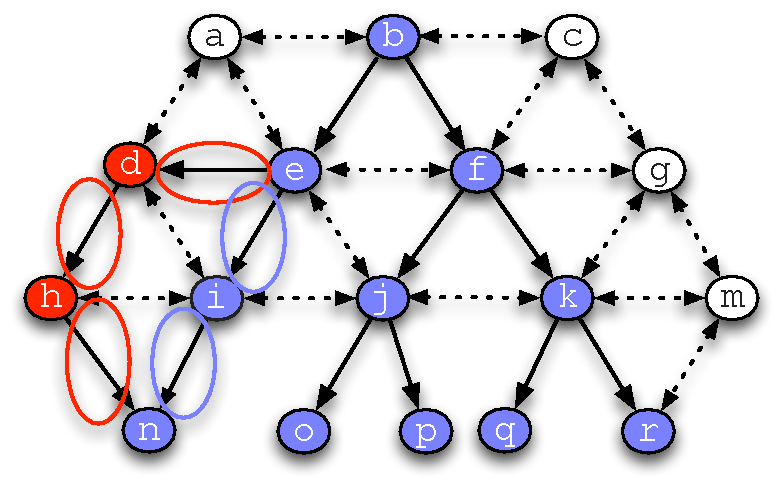
\includegraphics[scale=0.51]{figs/min-control-directed-example.pdf}
%\caption{Primary tree $T^l$ and backup tree, $\hat{T}^l$, where $l=(e,i)$. Edges unique to $T^l$ are circled in blue and unique $\hat{T}^l$ edges are circled in red. 
%$V^l \setminus \hat{V}^l = \{i\}$ and $\hat{V}^l \setminus V^l = \{d,h\}$. }
%\label{fig:min-control-example}
%\end{figure}


{\bf \pre \textsc{Algorithm.}}
\pre computes and installs backup tree flow entries \emph{before} a primary tree link, $l$, fails.  After $l$ fails, \pre signals the backup tree root
to install a forwarding rule that activates the backup tree.  We use the term ``activate'' to mean packets are multicasted using the backup tree rather than the primary tree.

%as opposed to \post that requires signaling multiple nodes to install a backup tree, \pre yields faster recovery than \posts. 

\pre cannot, without modifications, pre-install basic flow entries at all nodes because incorrect forwarding would result. Doing so at a node, $d$, common to the primary and backup tree
where the backup and primary tree have different outgoing links would either result in packets erroneously forwarded at $d$ using the backup tree before a link failure occurs or 
incorrectly forwarding packets using the primary tree after the link failure. 
We say that $d \in D^l$, where $D^l$ contains each node with one or more outgoing links in $T^l$ and one or more outgoing links in $\hat{T}^l \setminus T^l$.
Revisiting the Figure \ref{fig:intuition-example} example, installing a $\hat{T}_c$ forwarding rule at $g$ and $m$ before $(g,l)$ fails would be problematic for the reasons just described.

%Because $e$ has an outgoing link $(e,i) \in T^l$ and another outgoing link $(e,d)$ unique to $\hat{T}^l$,
%pre-installing $\hat{T}^l$'s flow entry at $e$ would cause incorrect forwarding for either $T^l$ or $\hat{T}^l$.  
%We say that $e \in D^l$, where $D^l$ contains each node with one or more outgoing links in $T^l$ and one or more outgoing links in $\hat{T}^l \setminus T^l$.

%{\it [TODO: Missing description of how root node is signaled to write the {\tt bid}. ]}

To address this issue, \pre assigns a unique \emph{backup tree id}, denoted {\tt bid}, to each backup tree.  For each $d \in D^l$, the flow entry matches and forwards packets
using the {\tt bid} value written in the {\tt dl\_src} field. When the backup tree $\hat{T}^l$ is activated, \pre writes the {\tt bid} in the
{\tt dl\_src} packet header field, indicating that these packets should be disseminated by $\hat{T}^l$ rather than $T^l$.
In more detail, \pre preinstalls and activates $\hat{T}^l$ using the following steps, where we assume $\hat{T}^l$ has {\tt bid=AA}:
\begin{enumerate}
	%\item Computes $D^l$.
	
	\item At each $d \in D^l$, \pre pre-installs a flow entry matching packets using $\hat{T}^l$'s multicast address, {\tt dl\_src = AA}, and wildcards for all other match fields. 
	%\footnote{We assume $T^l$ has multicast address \mdsts.}
	
	\item Preinstalls a basic flow entry at each $b \in B^l \setminus D^l$.

	\item When it is detected that $l$ fails, \pre installs a rule at the $\hat{T}^l$ root node that writes {\tt AA} in the {\tt dl\_src} header field of each $\hat{T}^l$ packet.
	%$e_r$ is given a higher priority than any other rule installed at $r$.
\end{enumerate}

For $\hat{T}_c$ in Figure \ref{fig:intuition-example}, \pre pre-installs a forwarding rule at $m$ that matches packets using $\hat{T}_c$'s {\tt bid}, {\tt CC}, and $T_c$'s multicast 
address.  After $(g,l)$ fails, \pre signals $c$ to write {\tt CC} in the {\tt dl\_src} header field of each $\hat{T}_c$ packet.  As a result, packets at $m$ are correctly forwarded to $l$,
$n$, and $t$.

{\bf Comparing \pre and \posts.}
Since \pre must signal only a single node, as opposed to multiple nodes with \posts, to install a backup tree, \pre is fast. However, \pres's speed comes at the cost of 
storing a potentially large number of flow entries at the switches, especially since \mdr computes, for each primary tree, a backup tree for each primary tree link. \post, on the other hand,
only installs backup tree flow entries after a link failure is detected.
These trade-offs are studied in Section \ref{sec:evaluation} using simulations.

%\post installs backup tree forwarding rules after a link failure is detected, while \pre installs backup tree flow entries before a link failure occurs. With \pres, the backup 
%trees are only activated -- by writing an identifier in each packet header signaling packets to be routed using the backup tree -- after the link failure is detected.

%\pre requires that only the root node needs to be signaled to install a backup tree, at the cost of storing unused flow entries (i.e., backup tree flow entries installed before link 
%failures occur).  In contrast, because backup tree flow entries are not preinstalled, \post introduces no storage overhead. However, multiple nodes must be signaled 
%to install a backup tree with \posts.
%and does not need tree ids to differentiate between primary tree and backup tree flow rules. % However, this comes at the cost of signaling overhead as each $B^l$ node must be signaled.




\subsection{Garbage Collection}
\label{subsec:garbage}

After a link fails, primary tree forwarding rules may become stale. \mdrs's garbage collection routine identifies and deletes these stale flow entries. 
Because garbage collection is not needed for correct data dissemination, garbage collection is run when necessary to free switch flow table space. 
%Note that this is not as simple as deleting all flow entries of each primary tree using $l$, $T^l$, because a backup tree may be reusing one of these flow entries. 

Garbage collection is straightforward, but more involved than simply deleting all flow entries of each primary tree, $T^l$, using $l$.  Doing so would be problematic 
because a backup tree may be reusing one of these flow entries.  To address this, \mdr maintains a dictionary, {\tt rule\_map}.  For each node, $v$, {\tt rule\_map} records
each flow entry installed at $v$ and the multicast trees using the flow entry. %each multicast tree (primary tree and backup trees) using $v$ to the flow entry installed at $v$. 
When $l$ fails, the garbage collection routine determines the set of stale forwarding rules for each $T^l_i \in T^l$ by consulting  {\tt rule\_map}.
A stale rule exists at each $v \in V_i \setminus \hat{V}_i^l$ (i.e., nodes unique to the primary tree) and each $d \in D_i^l$ (nodes where the backup tree diverges from the primary tree).
%Based on this criteria, \mdr consults {\tt rule\_map} to find all stale flow entries.
Finally, each stale forwarding rule is either explicitly removed (if using a hard state signaling protocol \cite{Ji03}) 
or \mdr allows the forwarding rule to timeout (if using a soft state signaling algorithm \cite{Clark88}).



%Under our \base multicast implementation, garbage collection is straightforward.  
%\mdr maintains a dictionary, {\tt rule\_map}, for each node, mapping each multicast tree (primary tree and backup trees) using $v$ to the flow entry installed at $v$.
%When a link, $l$, fails the garbage collection routine determines the set of stale forwarding rules for each $T^l_i$. 
%A stale rule exists at each $v \in V_i \setminus \hat{V}_i^l$ (i.e., nodes unique to the primary tree) and each $d \in D_i^l$ (nodes where the backup tree diverges from the primary tree).
%The controller consults {\tt rule\_map} to find the forwarding rule at each node and either sends an explicit remove flow message to each of these nodes (if using a hard state signaling 
%scheme \cite{HardSoftState}) or allows the forwarding rule to time out (with a soft state algorithm \cite{HardSoftState}).



\subsection{Optimized Multicast Implementation}
\label{subsec:merge}

% REVISED STRUCTURE: (a) merger is optimization to \base.  given a set of directed trees, \merge produces small set of fwd rules.  apply to PTs and backup trees, to get less control 
% 		state and faster install.  (b) basic inefficiency, the example,  (c) outline of section
As an optimization to the \base multicast implementation, described in Section \ref{subsec:openflow}, we present the \merge algorithm.  
Given a set of directed trees, produces a near-minimum set of OpenFlow forwarding rules by
consolidating flow table entries at each node where multiple trees use the same set of out-links.  \merge reduces the control state (i.e., number of forwarding rules) necessary to 
multicast packets and, when applied to installing backup trees, can yield faster recovery since fewer control messages are needed to activate backup trees.



%\merge can significantly reduce the control state associated with a multicast tree. At noted in Section \ref{subsec:openflow}, space efficiency is important because OpenFlow switches 
%can only support a limited number of flow table entries.
%Additionally, \merge can yield faster recovery when backup trees are installed using \posts.  Fewer backup tree flow table entries translates to fewer control messages to activate backup trees.

In the next section (\ref{subsubsec:merge-motivate}), we motivate the need for \merge by showing some of the inefficiencies of \bases.  Next, Section \ref{subsubsec:merge-primary} 
presents a simplified version of  \merge that considers only primary trees.  Then, we extend
\merge in Section \ref{subsubsec:merge-backup} to account for backup trees.  Section \ref{subsubsec:merge-discuss} concludes the section with a discussion of how \merge affects garbage
collection and \pcnts, along with informal commentary on its optimality.
%optimality, and complexity.

\begin{figure}
  \centering
   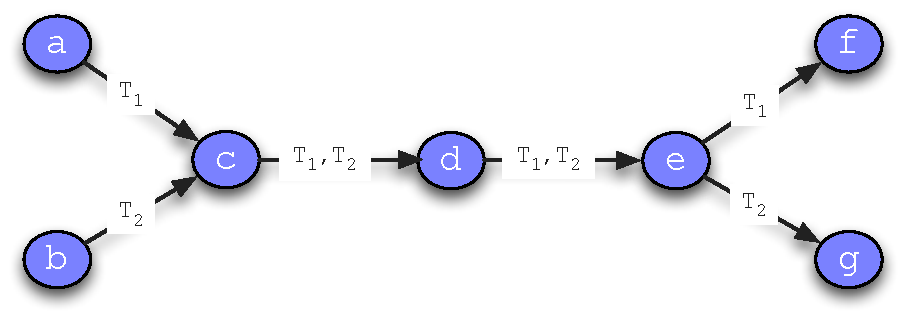
\includegraphics[scale=0.55]{figs/merger-example.pdf}
\caption{Example showing a subtree of two multicast trees, $T_1$ and $T_2$.  The edges used by each multicast tree are marked.}
\label{fig:merger-example}
\end{figure}


\subsubsection{Motivation: \basen Algorithm Inefficiencies}
\label{subsubsec:merge-motivate}

The \base multicast implementation creates a flow table entry at each node of a multicast tree that matches using the tree's multicast address. 
As a result, a switch, $v$, may have multiple flow table entries executing the same actions.  This occurs when multicast trees share the same outgoing links at $v$. 
\footnote{In cases where the tree can either be a primary tree or backup tree, we refer to the tree as a multicast tree.}
These inefficiencies are the motivation for developing the \merge algorithm, which replaces the set of flow table entries \base would create at $v$ with a single flow table entry. 
To do so, \merge writes a common identifier, or tag, in packet headers at the node immediately upstream from $v$. Using this tag, \merge creates a \emph{single} rule at $v$ to match and 
forward packets of \emph{all} trees with the same outgoing links at $v$.

Consider the simple example shown in Figure \ref{fig:merger-example} with two multicast trees $T_1$ and $T_2$. The directed links used by each tree are marked.
\base creates a flow table entry for $T_1$ at $a$, $c$, $d$, $e$, and $f$ and a flow table entry at $b$, $c$, $d$, $e$, and $g$ for $T_2$.  Because 
$T_1$ and $T_2$ both use the same outgoing links at $c$ and $d$, only a single forwarding rule is needed at each node.  This is what \merge creates and in the next two sections we describe how.

%In contrast, \merge leverages that $T_1$ and $T_2$ both use the same outgoing links at $c$ and $d$ to replace the two separate flow table entries at $c$ and $d$, created under \bases, with a single 
%forwarding rule. To do so, \merge first creates an action at $a$ and $b$ to write an identifier in the packet headers of all packets traversing $(a,c)$ and $(b,c)$.
%Then, at $c$ and $d$, \merge creates a single rule to match and forward packets based solely on this tag.




\subsubsection{\mergen Algorithm for Primary Trees}
\label{subsubsec:merge-primary}


\merge consolidates flow table entries at each node, $v$, where multiple primary trees share the same outgoing links. 
Upstream from $v$, \merge writes an identifier, or \emph{tag}, in packet headers and uses this tag to match packets at $v$ using a single rule shared by each of these primary trees.
%An identifier, or \emph{tag}, is used to match packets at $v$.  
%\merge writes this tag in the packet header at the node immediately upstream from $v$. % in the packet header of all packets corresponding to any of these multicast trees. 
The tag is removed downstream from $v$ where the trees diverge. 

A tag is a globally unique Ethernet address \merge writes in a packet header's {\tt dl\_dst} field (i.e., the Ethernet destination address).  When possible, \merge flow table entries use 
tags to match and forward packets, meaning that packets are matched solely on their {\tt dl\_dst} value.
When the same Ethernet address is applied to the packets of more than one multicast tree, we refer to this as a \emph{group tag}.  A \emph{single tag} is an 
Ethernet address used by only one tree. We use the term \emph{tag} to generically refer to either a group or single tag.
%\footnote{In some cases, packets corresponding to a multicast tree $T_i$ already have a tag written in their packet header upon reaching node $u$.  If this same tag is used to match packets 
%at $d$ where $(u,d) \in T_i$ no action is created at $u$ to write this same tag. However, for ease of explanation, we say that \merge writes the tag at $u$.}

\begin{figure}
  \centering
   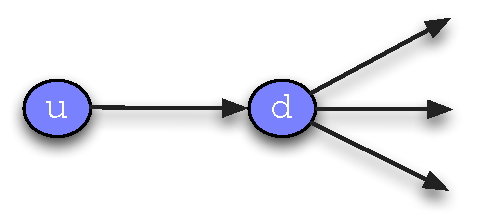
\includegraphics[scale=0.5]{figs/merger-ud.pdf}
\caption{Subgraph used to describe \merge in Section \ref{subsubsec:merge-primary}.}
\label{fig:merger-ud}
\end{figure}

%With these preliminaries in place, 
We are now ready to describe \merge in more detail.  
First, \merge marks the edges used by each primary tree.  Then, \merge executes a breadth first search of each primary tree, $T_i$, starting at its root.  
For each link $(u,d) \in T_i$ as shown in Figure \ref{fig:merger-ud}, \merge determines the match pattern to create at $d$ and the tagging actions to apply at $u$ using the following steps:
\footnote{Because $T_i$ is a tree, $(u,d)$ must be its only incoming link to $d$.  Therefore, we can determine $T_i$'s locally optimal tagging rule at $d$ by only considering $u$ and $d$.}
\begin{enumerate}

	\item Finds the set of trees, $S$, using $(u,d)$ that share the same outgoing links as $T_i$ at $d$. 

	\item If $|S| \geq 1$, \merge creates an action to write a group tag at $u$.  For each $T_j \in S \cup \{T_i\}$, \merge finds the rule at $u$ used to forward $T_j$ and appends an action
	to write a group tag to the rule's action list.
	Then, a single rule is created at $d$ that matches packets using this group tag and has an initial action list forwarding packets out the appropriate ports.

	\item If $S = \emptyset$, \merge peaks upstream at $u$ to determine whether to use a single tag or $T_i$'s multicast destination address to match $T_i$'s packets at $d$. 
	When $T_i$ is matched using either a single tag or its multicast destination address at $u$, \merge creates a rule at $d$ to match packets using a single tag and writes this single
	tag at $u$.  Otherwise, \merge creates a rule at $d$ matching packets using $T_i$'s multicast destination address (no action is needed at $u$).  
	%\footnote{If we were to write $T_i$'s single tag at $u$, this tag would be erroneously be applied to any other multicast tree using the same group tag as $T_i$ to match packets at $u$. }
	%Only when $T_i$ is matched using either a single tag or its multicast destination address at $u$, do we create a rule at $d$ to match packets using $T_i$'s single tag.  In which case, 
	%an action is created at $u$ to write this single tag.

\end{enumerate}
In step (3), we aim to use single tags to match packets because they allow \emph{any} backup tree to reuse $T_i$'s rule at $d$ by simply writing this tag at $u$.  
Whereas, if $T_i$'s multicast address is used to match packets at $d$, only $T_i$'s backup trees can reuse this forwarding rule (since $T_i$'s multicast address is unique to its multicast group).
We comment further on this design decision in the next section.

%In the Figure \ref{fig:merger-example} example, \merge leverages that $T_1$ and $T_2$ both use the same outgoing links at $c$ and $d$ to create a single rule at each node (as opposed
%to two separate flow table entries that would be created with \bases).  %After marking the edges used by $T_1$ and $T_2$, \merge
In the Figure \ref{fig:merger-example} example, \merge  creates an action at $a$ and $b$ to write a group tag in the packet headers of all packets traversing $(a,c)$ and $(b,c)$.
Then, at $c$ and $d$, \merge creates a single rule to match and forward packets based solely on this tag.  With regard to the breadth-first search (BFS) described earlier, 
\merge executes the following steps in  its breadth-first search (BFS) of $T_1$ at nodes $c$, $d$, and $e$.
%We describe the steps \merge executes in its breadth-first search (BFS) of $T_1$ at nodes $c$, $d$, and $e$.
At $c$, $S=\{T_2\}$ so \merge finds $T_1$'s rule at $a$ and includes an action to write a group tag, {\tt 12}, in all packets sent out $a$'s port to $c$. 
Then, \merge creates a flow table entry at $c$ that matches packets with {\tt dl\_dst = 12} and forwards packets out the port to $d$.  The same set of actions occur when the BFS reaches $d$. 
%except that no group tag needs to be written at $c$ because the same group tag
%At $e$, $S=\emptyset$ because $T_1$ and $T_2$ diverge. at $e$.  
\merge creates a forwarding rule at $e$ that matches packets using $T_1$'s multicast address and forwards these packets to $f$.



\subsubsection{\mergen Algorithm for Backup Trees}
\label{subsubsec:merge-backup}

Having discussed \merge for the primary tree case, we are now ready to extend \merge to generate forwarding rules for backup trees.  \merge 
aims to reuse forwarding rules of primary trees because these rules are already installed in the network, allowing the installation algorithm
(e.g., \pre or \posts) to avoid installation a new forwarding rule.  In cases where primary tree rules cannot be reused, \merge consolidates
flow table entries with other backup trees that have common forwarding behavior.

%We describe the case of generating forwarding rules for a set of backup trees, $\hat{T}^l$, using $l$. 
For a set of backup trees, $\hat{T}^l$, \merge generates backup tree forwarding rules as follows. 
\merge executes two rounds of BFS, traversing all
$\hat{T}^l_i \in \hat{T}^l$ in each round.  In the first round, for each $\hat{T}_i^l$, \merge finds each node where $\hat{T}_i^l$ has the same outgoing links as a primary tree.  
If so, $\hat{T}_i^l$ reuses the primary tree flow table entry at this node, $v$: \merge writes the primary tree tag at $v$'s parent node
allowing $\hat{T}_i^l$ packets to be forwarded using the primary tree rule, and makes no changes at $v$.

In the second round of BFSs, \merge consolidates flow table entries among the other backup trees for $l$
at nodes where primary tree tag reuse was not possible.  
To do so, the algorithm from Section \ref{subsubsec:merge-primary} is executed but comparing $\hat{T}_i^l$'s outgoing links with the outgoing links of 
each $\hat{T}_j^l \neq \hat{T}_i^l$ at nodes where $\hat{T}_i^l$ and $\hat{T}_j^l$ were unable to reuse primary tree tags. 

When \merge is applied to \pre and \post (referred to as \pres+\merge and \posts+\merges) the tag becomes the sole match criteria used by its flow table entry, with one exception.  This 
occurs with \pres+\merge when a {\tt bid} is required to distinguish between a backup and primary tree, as described in Section \ref{subsec:install-backups}. In those cases, the 
{\tt bid} and {\tt dl\_dst} fields are both used as match criteria.

%\merge attempts to reuse flow table entries of primary trees already installed in the network that share forwarding behavior with a backup tree. 
%First, \merge attempts to reuse flow table entries of primary trees already installed in the network that share forwarding behavior with a backup tree.  At nodes where this possible, no 
%flow table entry needs to be installed.  At the remaining nodes, % At nodes where this is not possible,
%\merge applies the procedure from Section \ref{subsubsec:merge-primary} to consolidate forwarding rules with other backup trees.  We detail these steps below. % for backup trees of link $l$.



%Under \merge we can avoid matching using a tree-id at any $d \in D^l_i$ where $\hat{T}_i^l$ uses a group tag or reuses a primary tree tag. 
%These tags are applied upstream from $d$ and are different from any tags $T_i^l$ uses  a $d$.  The tree-id is only required at $d \in D^l_i$ where \merge is forced to 
%match $\hat{T}_i^l$'s multicast address or single tag.  \merge described in Section \ref{subsec:merge-backup}, is modified to incorporate this additional match criteria. 

\subsubsection{\mergen Discussion}
\label{subsubsec:merge-discuss}

%Now that we have presented the core of aspects of \merges, we comment on. We comment on a number of 
To unify our presentation of \merges, we comment on some of the properties of the algorithm along with the implications of using \merge on other important aspects of \mdrs.
%In the following order, we discuss the advantages of using \merges, \merge time complexity, \merges's implications on garbage collection, \merges's ``do not harm'' property, and
%how \pcnt monitors \merge flows. 

{\bf Benefits.}
In comparison with \bases, \merge reduces the number of forwarding rules required to install each multicast tree.  As a result,
\merge is more space efficient and can yield faster backup tree installation.
%By reducing the number of forwarding rules required to install each multicast tree, \merge is more space efficient and can yield faster backup tree installationi with \posts+\merges.
Recall that for each primary tree, \mdr pre-computes a backup tree for each of its links.  In this scenario \pres+\merge can significantly reduce the number of pre-installed rules.
These savings are especially important because, as noted in Section \ref{subsec:openflow}, OpenFlow switches can only support a limited number of flow table entries.
With \posts, \merge can yield faster recovery because fewer backup tree flow table entries translates into fewer control messages to activate backup trees.

{\bf Time Complexity.}
Like \bases, \merge complexity is bounded by the breadth-first search (BFS) executed for each of the $m$ multicast trees given as input.  At each node, $v$, visited in the BFS, \merge
compares the out-links used by all other multicast trees that use $v$.  Since there can be at most $m$ such trees, this takes $O(m)$ time.  If we let $n$ be the number of graph nodes,
each BFS takes $O(mn)$ time \footnote{BFS has $O(|V|+|E|)$ complexity. In our case, each BFS is over a directed tree, meaning the number of edges traversed in each BFS is $O(n-1)$.  
Therefore, we can simplify BFS time complexity to $O(n)$.}
and the total time complexity of \merge is $O(m^2n)$.

% O( V+E), is O(V) because we are dealing with trees
% each BFS step has O(m) complexity, since need to check the out-links of all other trees using v
%  m x O(mn) -- O(m^2n)

{\bf Garbage Collection}.
\mdrs's garbage collection algorithm remains unchanged from the description in Section \ref{subsec:garbage}.  
Recall that {\tt rule\_map} is a dictionary that maps the flow table entry installed at each node to the
set of backup and primary trees using the flow table entry. The only difference between \base and \merge garbage collection is the number of stale rules it identifies (likely fewer
stale rules with \merges) not how the stale rules are found.  
As with \bases, \merge garbage collection can find any stale forwarding rules by consulting {\tt rule\_map}.


%Garbage collection
%Under our \base multicast implementation, garbage collection is straightforward.  The controller maintains a dictionary, {\tt rule\_map}, for each node, mapping
%each multicast tree (primary tree and backup trees) using $v$ to the flow table entry installed at $v$. When a link, $l$, fails the garbage collection routine determines 
%the set of stale forwarding rules for each $T^l_i$. A stale rule exists at each $v \in V_i \setminus \hat{V}_i^l$ (i.e., nodes unique to the primary tree) and each $d \in D_i^l$ 
%(nodes where the backup tree diverges from the primary tree).  The controller consults {\tt rule\_map} to find the forwarding rule at each node and either sends an explicit 
%remove flow message to each of these nodes (if using a hard state signaling scheme \cite{HardSoftState}) or allows the forwarding rule to time out (with a soft state algorithm \cite{HardSoftState}).

%With \merges, garbage collection adds an additional check before removing any candidate stale flow table entry, $c_v$, found using the procedure described in the previous paragraph.  
%Garbage collection consults {\tt rule\_map} to determine if any other primary tree or newly installed backup tree uses $c_v$, if so 
%is modified to check that no other primary tree 

%\merge complicates garbage collection because it is no longer the case that an installed flow table entry is used by a single multicast tree (e.g., multiple primary trees
%can share the same flow table entry).  Garbage collection must now consider that a different set of primary trees
%use flow table entry, $e$, before $l$ fails versus after $l$ fails and backup trees $\hat{T}^l$ are installed.  To account for this, we modify the first step of garbage collection.  
%Rather than simply add $T_i$'s flow table entry, $e_v$, at each $v$ to $E_r$, the garbage collection first checks if any newly installed tree (i.e., each tree in $\hat{T}^l$) reuses $e_v$. Then, we
%check if any primary tree unaffected by $l$ failing (i.e., each tree in $\bar{T}^l$) uses $e_v$. If either of these checks is positive, $e_v$ is 
%not included in $E_r$ but {\tt flow\_map} is updated for $T_i$.  Otherwise, $e_r$ is added to $E_r$ and {\tt flow\_map} is updated for $T_i$.

%\item \underline{Garbage Collection}: keep track of flows used by each tree.  garbage collection ensures flows of unaffected trees are not removed.

{\bf Do No Harm.} 
We say that \merge is an algorithm that does ``no harm''  \footnote{This is similar in spirit to the Hippocratic Oath taken by physicians that they will ``never do harm [to patients]'' }
because (a) \merge never creates more flow table entries than \base and (b) when generating rules for backup trees, \merge makes no modifications to flow table entries of primary trees that do not use the 
failed link. We informally prove each of these properties below.

Regarding (a), consider an arbitrary multicast tree (primary of backup tree), $T_i$. \merge creates at most one flow table entry at any $v \in T_i$.  
The flow table entry, $e_i$, either matches and forwards packets using a group tag, a single tag, or using the $T_i$'s multicast address.  Any $e_i$ tagging actions 
are simply appended to $e_i$'s action list (when \merge visits $T_i$'s children of $v$), requiring the creation of no additional flow table entries.  We conclude that in the worst case,
\merge creates the same number of flow table entries as \bases.  

Now consider property (b) where we let $T_j$ refer to a primary tree not using $l$. By construction, \merge only creates flow table entries and new actions for the backup trees of 
link $l$ (i.e., $\hat{T}^l$). These flow table entries have distinct match criteria than those \merge creates for $T_j$.  If a backup tree reuses $T_j$'s flow table entry at $v$, 
no changes are made to this flow table entry.  Lastly, \mdrs's garbage collection algorithm ensures that no $T_j$ flow table entry is removed.

%As an aside, \merges's do no harm property ensures that under \merges, garbage collection has fewer flow table entries to remove than with \bases.  Intuitively, this 
%is reasonable because \merge seeks to reuse primary tree flow table entries. 


{\bf Optimality}.  
Because \merge makes tagging decisions locally at each node, $v$, based only on the multicast trees using $v$'s outgoing links and the tags used at $v$'s parent nodes,
\merge does not always yield the minimum set of forwarding rules.
Consider again Figure \ref{fig:merger-example} but replace $T_1$ with $S_1$ and $T_2$ with $S_2$, where $S_1$ and $S_2$ are sets of multicast trees of size $k$.
%$S_1=\{T_1,T_2,...,T_k\}$ and $S_2 = \{T_{k+1},T_{k+2},...,T_{2k+1}\}$.  
In this scenario, \merge writes the same group tag, denoted {\tt 12}, at $a$ and $b$ for each tree in $S_1$ and $S_2$.  Then, at $c$ and $d$ \merge installs a single rule that matches and forwards 
using the {\tt 12} tag.  Lastly, for each $T_i \in S_1 \cup S_2$, a rule is created at $e$ that matches packets using each $T_i$'s multicast address.  %This results in 

A better solution in this example is to use a different group tag for $S_1$ and $S_2$.  Under this proposal, let {\tt 11} be the group tag applied to each tree in $S_1$ 
at $a$ and {\tt 22} the tag we write 
in the packet header of each tree in $S_2$.  These group tags can be used create two separate rules at $c$, $d$, and $e$ to forward $S_1$ packets based on {\tt 11} and $S_2$ packets using {\tt 22}.
By using different tags for $S_1$ and $S_2$, we avoid having to create $2k$ separate rules for each tree in $S_1 \cup S_2$ at $e$, clearly a better solution that the 
one produced by \merges. 

This example suggests that an algorithm, $\mathcal{A}$, that finds the minimum number of forwarding rules for a set of multicast trees $T$ 
must consider, for $S \subseteq T$ where each multicast tree $S_i \in S$ uses link $(u,d)$, how each of $S$'s subsets share links downstream from $d$.
Since this requires computing the power set of $S$ and there are an exponential number of ways $S$'s subsets can use common links downstream from $d$,
we conjecture that no polynomial time $\mathcal{A}$ exists. %a polynomial time algorithm that yields the optimal  solution does not exist.





%The single group tag used at u forces a separate rule to be created for each tree in S if not all S have the same outports at d.  In some cases, it is beneficial to partition S into subsets, 
%based on links shared downstream, and use a group tag unique to each subset to match and forward packets downstream. 

%Consider the following example.  S_1 and S_2 denote a set of trees and let S = S_1 \cup S_2.   Merger creates an action at a and b to write group tag, denoted 12,  for each tree in S_1 and S_2.  Then, at u a single rule matches and forwards using the 12 tag.  Lastly, a rule is created at d for each tree in S that matches using the tree's destination address to ensure correct forwarding at d.  A better approach is to write group tag 11 at a for S_1 and group tag 22 for S_2 at b.   We can use these group tags to match and forward -- using two separate rules -- at u and d using group tags 11 and 22.   Using different tags for S_1 and S_2 makes it unnecessary to create a separate rule for each tree in S at d.   The same challenge arises if u and d were connected using additional links all used by S. 

{\bf Implications for \pcnts.}
\pcnt requires no changes to monitor packet loss of flows forwarded using \merge rules. However, we make 
the case here that \merge can improve the accuracy of \pcnt loss rate estimates and reduce the time to compute these estimates.  In Section
\ref{subsec:eval-pcount}, we will find that our simulations bear out the qualitative argument made here.

% (a) can tune k.  cost associated with each k
Recall from Section \ref{subsec:pcnt} that with \pcnt the number of monitored flows, $k$, can be tuned.
Determining an appropriate $k$ parameter involves a trade-off between the accuracy of packet loss estimates and time: larger $k$ yield more accurate packet loss estimates
but at the cost of slower detection times (the time between when packet loss occurs and when it is detected). Detection times of a monitored link, $(u,d)$, increase with larger $k$
for two reasons. One, for each of the $k$ flows, \pcnt makes a copy of the flow's forwarding rule at $u$ and $d$ in order tag and count packets.  Two, 
\pcnt sends $k$ queries to $u$ to read the state of each flow table entry generated by \pcnts. % generated flow table entry and a single aggregate statistic query to $d$.

%a function of the number of statistic queries \pcnt sends. % to the switches of a monitored link.  
%Recall from Section \ref{subsec:pcnt}, when estimating packet loss of a link, $(u,d)$, \pcnt makes a copy of the flow table entry at $u$ and $d$, for each flow \pcnt monitors. 

With \merge the same flow table entry, $e_i$, can be used by multiple ($r$) flows.  In these cases, \pcnt only needs to explicitly monitor one of these flows to measure
the packet loss of all $r$ flows.  That is, \pcnt can monitor the loss of all $r$ flows with cost of monitoring a single flow:
the one copy of $e_i$ \pcnt makes at $u$ and $d$ ensures that packets of any of these $r$ flows are tagged and counted and
only a single statistic query is needed to retrieve $e_i$'s packet count.

Consider the example in Figure \ref{fig:intuition-example-t1} and suppose that \pcnt monitors link $(g,l)$. 
Two multicast flows -- $f_b$ for primary tree $T_b$ and $f_c$ for primary tree $T_c$ -- traverse
$(g,l)$.  \base creates a separate forwarding rule for $f_b$ and $f_c$ at $g$ while \merge generates a single forwarding rule at $g$ used by both $f_b$ and $f_c$.  As a result, 
with \merges, \pcnt can track the  packet loss of $f_b$ and $f_c$ by querying just the shared \merge forwarding rule at $g$ (rather than interact with two separate \base forwarding rules).
These savings are quantified using simulations in Section \ref{subsec:eval-pcount}.

%Recall from Section \ref{subsec:pcnt} that with \pcnt the number of monitored flows, $k$, can be tuned.  Determining an appropriate $k$ parameter involves a trade-off between the accuracy of
%packet loss estimates and time: larger $k$ yield more accurate packet loss estimates but at the cost of slower detection times (the time between when packet loss occurs and when it is detected).
%Detection times of a monitored link, $(u,d)$, are a function of the number of statistic queries \pcnt sends. % to the switches of a monitored link.  
%\pcnt sends a read state query for each monitored flow to $d$ and a single statistic query to $d$.

%As a mechanism to count packet loss, \pcnt makes a copy of the flow table entry of each monitored flow where the flow table entry copy upstream tags packets upstream and a second flow table entry copy counts 
%tagged packets downstream.  Because with \merge the same flow table entry, $e_i$, may be shared by multiple flows, all of these flows can be monitored at the cost of monitoring a single flow: 
%only a single \pcnt statistic query is needed to retrieve $e_i$'s packet count rather than one separate query per flow using $e_i$ that would necessary with \bases.  




